\documentclass[11pt,a4paper]{report}
\usepackage[textwidth=37em,vmargin=30mm]{geometry}
\usepackage{calc,xunicode,amsmath,amssymb,paralist,enumitem,tabu,booktabs,datetime2,xeCJK,xeCJKfntef,listings}
\usepackage{tocloft,fancyhdr,tcolorbox,xcolor,graphicx,eso-pic,xltxtra,xelatexemoji}

\newcommand{\envyear}[0]{2025}
\newcommand{\envdatestr}[0]{2025-03-03}
\newcommand{\envfinaldir}[0]{webdb/2025/20250303/final}

\usepackage[hidelinks]{hyperref}
\hypersetup{
    colorlinks=false,
    pdfpagemode=FullScreen,
    pdftitle={Web Digest - \envdatestr}
}

\setlength{\cftbeforechapskip}{10pt}
\renewcommand{\cftchapfont}{\rmfamily\bfseries\large\raggedright}
\setlength{\cftbeforesecskip}{2pt}
\renewcommand{\cftsecfont}{\sffamily\small\raggedright}

\setdefaultleftmargin{2em}{2em}{1em}{1em}{1em}{1em}

\usepackage{xeCJK,xeCJKfntef}
\xeCJKsetup{PunctStyle=plain,RubberPunctSkip=false,CJKglue=\strut\hskip 0pt plus 0.1em minus 0.05em,CJKecglue=\strut\hskip 0.22em plus 0.2em}
\XeTeXlinebreaklocale "zh"
\XeTeXlinebreakskip = 0pt


\setmainfont{Brygada 1918}
\setromanfont{Brygada 1918}
\setsansfont{IBM Plex Sans}
\setmonofont{JetBrains Mono NL}
\setCJKmainfont{Noto Serif CJK SC}
\setCJKromanfont{Noto Serif CJK SC}
\setCJKsansfont{Noto Sans CJK SC}
\setCJKmonofont{Noto Sans CJK SC}

\setlength{\parindent}{0pt}
\setlength{\parskip}{8pt}
\linespread{1.15}

\lstset{
	basicstyle=\ttfamily\footnotesize,
	numbersep=5pt,
	backgroundcolor=\color{black!5},
	showspaces=false,
	showstringspaces=false,
	showtabs=false,
	tabsize=2,
	captionpos=b,
	breaklines=true,
	breakatwhitespace=true,
	breakautoindent=true,
	linewidth=\textwidth
}






\newcommand{\coverpic}[2]{
    % argv: itemurl, authorname
    Cover photo by #2~~(\href{#1}{#1})
}
\newcommand{\makeheader}[0]{
    \begin{titlepage}
        % \newgeometry{hmargin=15mm,tmargin=21mm,bmargin=12mm}
        \begin{center}
            
            \rmfamily\scshape
            \fontspec{BaskervilleF}
            \fontspec{Old Standard}
            \fontsize{59pt}{70pt}\selectfont
            WEB\hfill DIGEST
            
            \vfill
            % \vskip 30pt
            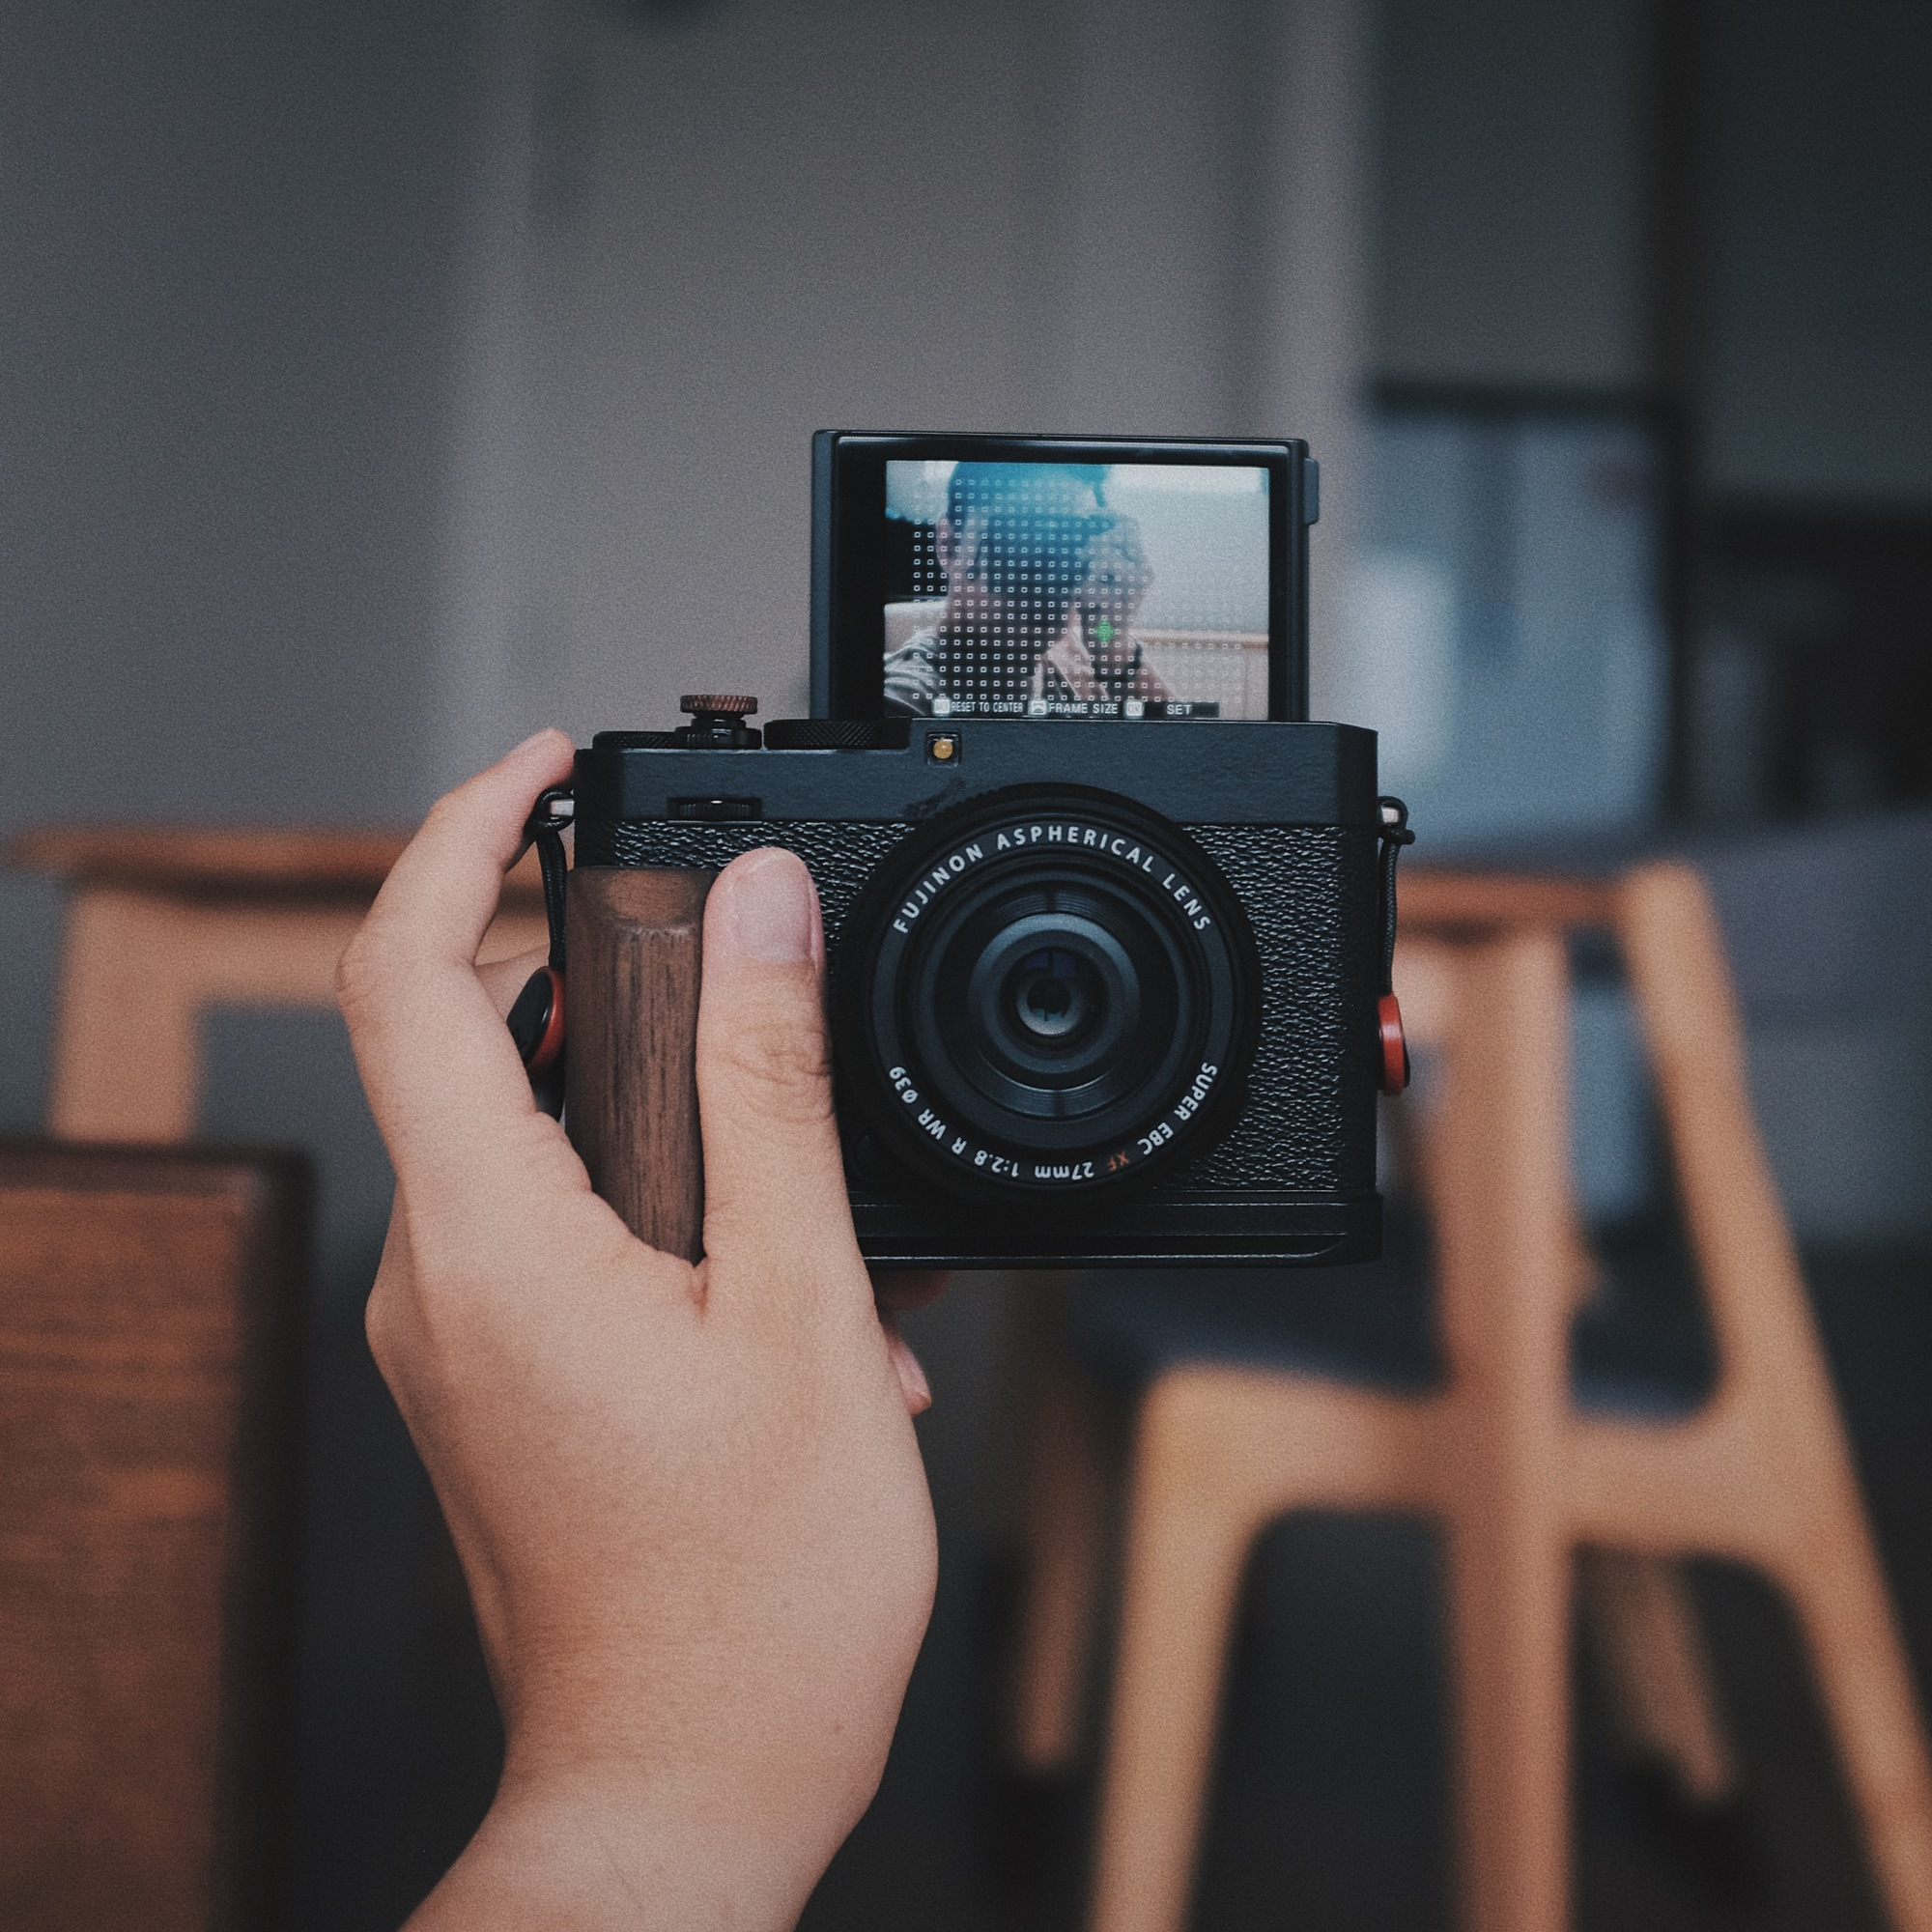
\includegraphics[width=\linewidth]{\envfinaldir/coverpic-prod.jpg}\par
            % \vskip 30pt
            \vfill

            \normalsize\rmfamily\scshape
            \copyright{} The Web Digest Project \hfill\large \envdatestr
        \end{center}
    \end{titlepage}
    % \restoregeometry
}
\newcommand{\simplehref}[1]{%
    \textcolor{blue!80!green}{\href{#1}{#1}}%
}
\renewcommand{\contentsname}{\center\Huge\sffamily\bfseries Contents\par\vskip 20pt}
\newcounter{ipartcounter}
\setcounter{ipartcounter}{0}
\newcommand{\ipart}[1]{
    % \vskip 20pt
    \clearpage
    \stepcounter{ipartcounter}
    \phantomsection
    \addcontentsline{toc}{chapter}{#1}
    % \begin{center}
    %     \Huge
    %     \sffamily\bfseries
    %     #1
    % \end{center}
    % \vskip 20pt plus 7pt
}
\newcounter{ichaptercounter}
\setcounter{ichaptercounter}{0}
\newcommand{\ichapter}[1]{
    % \vskip 20pt
    \clearpage
    \stepcounter{ichaptercounter}
    \phantomsection
    \addcontentsline{toc}{section}{\numberline{\arabic{ichaptercounter}}#1}
    \begin{center}
        \Huge
        \sffamily\bfseries
        #1
    \end{center}
    \vskip 20pt plus 7pt
}
\newcommand{\entrytitlefont}[1]{\subsection*{\raggedright\Large\sffamily\bfseries#1}}
\newcommand{\entryitemGeneric}[2]{
    % argv: title, url
    \parbox{\linewidth}{
        \entrytitlefont{#1}\par\vskip 5pt
        \footnotesize\ttfamily\mdseries
        \simplehref{#2}
    }\vskip 11pt plus 11pt minus 1pt
}
\newcommand{\entryitemGithub}[3]{
    % argv: title, url, desc
    \parbox{\linewidth}{
        \entrytitlefont{#1}\par\vskip 5pt
        \footnotesize\ttfamily\mdseries
        \simplehref{#2}\par\vskip 5pt
        \small\rmfamily\mdseries#3
    }\vskip 11pt plus 11pt minus 1pt
}
\newcommand{\entryitemAp}[3]{
    % argv: title, url, desc
    \parbox{\linewidth}{
        \entrytitlefont{#1}\par\vskip 5pt
        \footnotesize\ttfamily\mdseries
        \simplehref{#2}\par\vskip 5pt
        \small\rmfamily\mdseries#3
    }\vskip 11pt plus 11pt minus 1pt
}
\newcommand{\entryitemHackernews}[3]{
    % argv: title, hnurl, rawurl
    % \parbox{\linewidth}{
    %     \entrytitlefont{#1}\par\vskip 5pt
    %     \footnotesize\ttfamily\mdseries
    %     \simplehref{#3}\par
    %     \textcolor{black!50}{\href{#2}{#2}}
    % }\vskip 11pt plus 11pt minus 1pt
    \begin{minipage}{\linewidth}
            \entrytitlefont{#1}\par\vskip 5pt
            \footnotesize\ttfamily\mdseries
            \simplehref{#3}\par
            \textcolor{black!50}{\href{#2}{#2}}
    \end{minipage}\par\vskip 11pt plus 11pt minus 1pt
}







\begin{document}

\makeheader

\tableofcontents\clearpage




\ipart{Developers}
\ichapter{Hacker News}
\entryitemTwoLinks{2025 Hiring Pause}{https://news.ycombinator.com/item?id=43234153}{https://hr.cornell.edu/2025-hiring-pause}

\entryitemTwoLinks{Geothermal power is a climate moon shot beneath our feet}{https://news.ycombinator.com/item?id=43234089}{https://www.newyorker.com/news/the-lede/geothermal-power-is-a-climate-moon-shot-beneath-our-feet}

\entryitemTwoLinks{olduse.net}{https://news.ycombinator.com/item?id=43233305}{https://olduse.net/}

\entryitemTwoLinks{The Pentium contains a complicated circuit to multiply by three}{https://news.ycombinator.com/item?id=43233143}{https://www.righto.com/2025/03/pentium-multiplier-adder-reverse-engineered.html}

\entryitemTwoLinks{Speedrunners are vulnerability researchers, they just don't know it yet}{https://news.ycombinator.com/item?id=43232880}{https://zetier.com/speedrunners-are-vulnerability-researchers/}

\entryitemTwoLinks{Understanding Smallpond and 3FS}{https://news.ycombinator.com/item?id=43232410}{https://www.definite.app/blog/smallpond}

\entryitemTwoLinks{Executive wealth as a factor in return-to-office}{https://news.ycombinator.com/item?id=43232255}{https://twitter.com/EthanEvansVP/status/1895845734177452369}

\entryitemTwoLinks{Mark Cuban offers to fund former 18F employees}{https://news.ycombinator.com/item?id=43231062}{https://techcrunch.com/2025/03/01/mark-cuban-offers-to-fund-government-tech-unit-that-was-cut-in-the-middle-of-the-night/}

\entryitemTwoLinks{Show HN: I built a modern Goodreads alternative}{https://news.ycombinator.com/item?id=43230994}{https://kaguya.io/}

\entryitemTwoLinks{GPT-4.5: "Not a frontier model"?}{https://news.ycombinator.com/item?id=43230965}{https://www.interconnects.ai/p/gpt-45-not-a-frontier-model}

\entryitemTwoLinks{This Month in Ladybird February 2025}{https://news.ycombinator.com/item?id=43230920}{https://ladybird.org/newsletter/2025-02-28/}

\entryitemTwoLinks{Raspberry Pi Pico audio player}{https://news.ycombinator.com/item?id=43230821}{http://lucstechblog.blogspot.com/2025/02/raspberry-pi-pico-audio-player.html}

\entryitemTwoLinks{I struggled with Git, so I'm making a game to spare others the pain}{https://news.ycombinator.com/item?id=43230734}{https://initialcommit.com/blog/im-making-a-git-game}

\entryitemTwoLinks{Mozilla flamed by Firefox fans after reneging on promises to not sell their data}{https://news.ycombinator.com/item?id=43229668}{https://www.theregister.com/2025/03/02/mozilla\_introduces\_terms\_of\_use/}

\entryitemTwoLinks{German tourist held indefinitely in San Diego area immigrant detention facility}{https://news.ycombinator.com/item?id=43229475}{https://www.kpbs.org/news/border-immigration/2025/02/28/german-tourist-held-indefinitely-in-san-diego-area-immigrant-detention-facility}

\entryitemTwoLinks{Trust in Firefox and Mozilla Is Gone – Let's Talk Alternatives}{https://news.ycombinator.com/item?id=43229378}{https://boilingsteam.com/poll-trust-in-firefox-mozilla-is-gone/}

\entryitemTwoLinks{What, if anything, should I do about using Mozilla's Firefox}{https://news.ycombinator.com/item?id=43229267}{https://neilzone.co.uk/2025/03/what-if-anything-should-i-do-about-using-mozillas-firefox/}

\entryitemTwoLinks{The A.I. Monarchy}{https://news.ycombinator.com/item?id=43229245}{https://substack.com/home/post/p-156886169}

\entryitemTwoLinks{NIH.gov DNS servers down, making PubMed, BLAST, etc. unreachable [fixed]}{https://news.ycombinator.com/item?id=43229201}{https://www.nslookup.io/domains/www.nih.gov/dns-records/\#authoritative}

\entryitemTwoLinks{Crossing the uncanny valley of conversational voice}{https://news.ycombinator.com/item?id=43227881}{https://www.sesame.com/research/crossing\_the\_uncanny\_valley\_of\_voice}\ichapter{Phoronix}
\entryitemGeneric{\hskip 0pt{}Linux 6.14-rc5 Released: "Nothing Strange Stands Out"}{https://www.phoronix.com/news/Linux-6.14-rc5-Released}

\entryitemGeneric{\hskip 0pt{}NVIDIA Is Finding Great Success With Vulkan Machine Learning - Competitive With CUDA}{https://www.phoronix.com/news/NVIDIA-Vulkan-AI-ML-Success}

\entryitemGeneric{\hskip 0pt{}TurnkeyML 6.0 Released With OpenAI-Compatible Server, Other Changes}{https://www.phoronix.com/news/TurnkeyML-6.0-Released}

\entryitemGeneric{\hskip 0pt{}Steam Survey For February 2025 Shows A Big Drop To Linux Use}{https://www.phoronix.com/news/Steam-Survey-Feb-2025}

\entryitemGeneric{\hskip 0pt{}ARM Linux Kernel May Shift To Generic Entry Code: Less Assembly But Lower Performance}{https://www.phoronix.com/news/ARM-Linux-Generic-Entry}

\entryitemGeneric{\hskip 0pt{}SDL 3.2.6 Released With HiDPI Icons \& Color Management On Wayland}{https://www.phoronix.com/news/SDL-3.2.6-Released}

\entryitemGeneric{\hskip 0pt{}Linux's New Way Of Informing User-Space Over Hung GPUs May Become More Useful}{https://www.phoronix.com/news/Extending-Linux-GPU-Wedge-Event}

\entryitemGeneric{\hskip 0pt{}AMD Readies More Graphics Driver Improvements For Linux 6.15}{https://www.phoronix.com/news/AMDGPU-Linux-6.15-Round-2}

\entryitemGeneric{\hskip 0pt{}Intel Core 2 CPUs Have Been Affected By An Annoying Linux Kernel Bug For 5+ Years}{https://www.phoronix.com/news/Intel-Core-2-Stalls-Boot-Fix}\ichapter{Dribbble}
\entryitemGeneric{\hskip 0pt{}Star + Check Mark Icon Concept}{https://dribbble.com/shots/25698016-Star-Check-Mark-Icon-Concept}

\entryitemGeneric{\hskip 0pt{}Letter A}{https://dribbble.com/shots/25691267-Letter-A}

\entryitemGeneric{\hskip 0pt{}Tally Logo Design}{https://dribbble.com/shots/25693309-Tally-Logo-Design}

\entryitemGeneric{\hskip 0pt{}Detective Dog Logo}{https://dribbble.com/shots/25692587-Detective-Dog-Logo}

\entryitemGeneric{\hskip 0pt{}HyperSeed - Logo Design}{https://dribbble.com/shots/25692269-HyperSeed-Logo-Design}

\entryitemGeneric{\hskip 0pt{}Logo Design for Gaming Platform (Unused for Sale)}{https://dribbble.com/shots/25692257-Logo-Design-for-Gaming-Platform-Unused-for-Sale}

\entryitemGeneric{\hskip 0pt{}Barbershop app dashboard}{https://dribbble.com/shots/25687859-Barbershop-app-dashboard}

\entryitemGeneric{\hskip 0pt{}Ramotion Logo Design}{https://dribbble.com/shots/25582478-Ramotion-Logo-Design}

\entryitemGeneric{\hskip 0pt{}Cimet Stationery}{https://dribbble.com/shots/25687823-Cimet-Stationery}

\entryitemGeneric{\hskip 0pt{}Check Mark App Icon}{https://dribbble.com/shots/25687869-Check-Mark-App-Icon}

\entryitemGeneric{\hskip 0pt{}Block13 Promo Board Design}{https://dribbble.com/shots/25688403-Block13-Promo-Board-Design}

\entryitemGeneric{\hskip 0pt{}Letter a}{https://dribbble.com/shots/25680095-Letter-a}

\entryitemGeneric{\hskip 0pt{}auren - logo design}{https://dribbble.com/shots/25681046-auren-logo-design}

\entryitemGeneric{\hskip 0pt{}Block13 Skateboards \& Sreetwear}{https://dribbble.com/shots/25683504-Block13-Skateboards-Sreetwear}

\entryitemGeneric{\hskip 0pt{}Quokka Mascot}{https://dribbble.com/shots/25681470-Quokka-Mascot}

\entryitemGeneric{\hskip 0pt{}Cardi C}{https://dribbble.com/shots/25678066-Cardi-C}

\entryitemGeneric{\hskip 0pt{}R}{https://dribbble.com/shots/25673587-R}

\entryitemGeneric{\hskip 0pt{}Fitme home landing page}{https://dribbble.com/shots/25674639-Fitme-home-landing-page}

\entryitemGeneric{\hskip 0pt{}Unused Geometric Fox}{https://dribbble.com/shots/25677006-Unused-Geometric-Fox}

\entryitemGeneric{\hskip 0pt{}Triceratops Dino}{https://dribbble.com/shots/25676249-Triceratops-Dino}

\entryitemGeneric{\hskip 0pt{}Illustrated Icons - American Home Shield}{https://dribbble.com/shots/25666386-Illustrated-Icons-American-Home-Shield}

\entryitemGeneric{\hskip 0pt{}Tiger Style}{https://dribbble.com/shots/25676567-Tiger-Style}

\entryitemGeneric{\hskip 0pt{}Logo Tip 002. Rhythm in Logo Design}{https://dribbble.com/shots/25674872-Logo-Tip-002-Rhythm-in-Logo-Design}

\entryitemGeneric{\hskip 0pt{}The Business}{https://dribbble.com/shots/25676385-The-Business}


\ipart{Developers~~~~(zh-Hans)}
\ichapter{Solidot}
\entryitemGeneric{\hskip 0pt{}火星北极极冠年龄比预期的年轻}{https://www.solidot.org/story?sid=80688}

\entryitemGeneric{\hskip 0pt{}中国空间站将迎来巴基斯坦航天员}{https://www.solidot.org/story?sid=80687}

\entryitemGeneric{\hskip 0pt{}Slashdot日本语版``スラド''关闭1周年}{https://www.solidot.org/story?sid=80686}

\entryitemGeneric{\hskip 0pt{}微软将于 5 月 5 日关闭 Skype}{https://www.solidot.org/story?sid=80685}

\entryitemGeneric{\hskip 0pt{}AMD 宣布 RX 9000 系列显卡}{https://www.solidot.org/story?sid=80684}

\entryitemGeneric{\hskip 0pt{}长时间维护软件所面临的挑战}{https://www.solidot.org/story?sid=80683}

\entryitemGeneric{\hskip 0pt{}英国研究称散步有助于改善父女关系}{https://www.solidot.org/story?sid=80682}

\entryitemGeneric{\hskip 0pt{}暴力引发的基因表观遗传能持续数代}{https://www.solidot.org/story?sid=80681}

\entryitemGeneric{\hskip 0pt{}维苏威火山突然喷发致大脑组织玻璃化}{https://www.solidot.org/story?sid=80680}

\entryitemGeneric{\hskip 0pt{}过度种植抗根虫玉米会产生长期危害}{https://www.solidot.org/story?sid=80679}

\entryitemGeneric{\hskip 0pt{}日企计划 2027 年启动太空垃圾捕获试验}{https://www.solidot.org/story?sid=80678}

\entryitemGeneric{\hskip 0pt{}2024 年日本出生人数创历史最低}{https://www.solidot.org/story?sid=80677}

\entryitemGeneric{\hskip 0pt{}Microsoft Edge 准备淘汰 Manifest V2 扩展开始禁用 uBlock Origin}{https://www.solidot.org/story?sid=80676}

\entryitemGeneric{\hskip 0pt{}OpenAI 推出 GPT-4.5}{https://www.solidot.org/story?sid=80675}

\entryitemGeneric{\hskip 0pt{}Meta 解雇了约 20 名泄密的员工}{https://www.solidot.org/story?sid=80674}

\entryitemGeneric{\hskip 0pt{}EA 开源命令与征服系列游戏}{https://www.solidot.org/story?sid=80673}\ichapter{V2EX}
\entryitemGeneric{\hskip 0pt{}[程序员] [消费升级] 发帖扣 100+ 铜币}{https://www.v2ex.com/t/1115336}

\entryitemGeneric{\hskip 0pt{}[问与答] 咱同胞玩游戏能不能别作弊,真恶心。}{https://www.v2ex.com/t/1115335}

\entryitemGeneric{\hskip 0pt{}[分享创造] [送码] Forza Dash - 移动端的极限竞速地平线仪表盘}{https://www.v2ex.com/t/1115334}

\entryitemGeneric{\hskip 0pt{}[iPhone] 出 1 台加版 iPhone 16 PRO MAX 256G}{https://www.v2ex.com/t/1115333}

\entryitemGeneric{\hskip 0pt{}[旅行] 二月葡萄牙旅行小记}{https://www.v2ex.com/t/1115332}

\entryitemGeneric{\hskip 0pt{}[生活] 邻居在家干塑料制品,不定时会散发难闻的味道,想知道如何检测这个的危害。}{https://www.v2ex.com/t/1115331}

\entryitemGeneric{\hskip 0pt{}[Apple] 省电模式居然会影响 Wi-Fi 连接速率}{https://www.v2ex.com/t/1115330}

\entryitemGeneric{\hskip 0pt{}[分享发现] 突然发现 excalidraw 支持中文手写体了}{https://www.v2ex.com/t/1115329}

\entryitemGeneric{\hskip 0pt{}[问与答] 目前审查最低的在线大模型是?}{https://www.v2ex.com/t/1115328}

\entryitemGeneric{\hskip 0pt{}[程序员] 《中国税收居民身份证明》开具申请指南:适用于 Google AdSense 税务居住地证明及其他场景(最新)- 谷歌广告税务信息管理:如何申请办理税务居住地证明/中国税收居民身份证明}{https://www.v2ex.com/t/1115326}

\entryitemGeneric{\hskip 0pt{}[iPhone] iOS 端 AI 客户端求推荐}{https://www.v2ex.com/t/1115325}

\entryitemGeneric{\hskip 0pt{}[分享创造] ToyLLM: 学习为目的 LLM 库}{https://www.v2ex.com/t/1115324}

\entryitemGeneric{\hskip 0pt{}[分享创造] 试一试我做的 AI 修仙,分享一下游玩的感受}{https://www.v2ex.com/t/1115323}

\entryitemGeneric{\hskip 0pt{}[问与答] 国际课程 A-Level 资料求助}{https://www.v2ex.com/t/1115322}

\entryitemGeneric{\hskip 0pt{}[分享创造] 独立工具,提供电脑选配参考}{https://www.v2ex.com/t/1115321}

\entryitemGeneric{\hskip 0pt{}[分享创造] 快点 MJJ 导航-你的服务器购买指南}{https://www.v2ex.com/t/1115320}

\entryitemGeneric{\hskip 0pt{}[分享创造] [旅行 APP 产品诞生日记] 4day/100days}{https://www.v2ex.com/t/1115319}

\entryitemGeneric{\hskip 0pt{}[推广] Next.js (T3 Stack) Website Development}{https://www.v2ex.com/t/1115318}

\entryitemGeneric{\hskip 0pt{}[Apple] iOS 中孩子家庭账户绕过屏幕使用时间的方法}{https://www.v2ex.com/t/1115317}

\entryitemGeneric{\hskip 0pt{}[酷工作] SHEIN 内推}{https://www.v2ex.com/t/1115316}

\entryitemGeneric{\hskip 0pt{}[问与答] 有什么办法能统计公众号的总阅读量?}{https://www.v2ex.com/t/1115314}

\entryitemGeneric{\hskip 0pt{}[生活] 我想问问 有多少人是和爱情结婚的}{https://www.v2ex.com/t/1115313}

\entryitemGeneric{\hskip 0pt{}[创造者] [旅行 APP 产品诞生日记] 3day/100days}{https://www.v2ex.com/t/1115311}

\entryitemGeneric{\hskip 0pt{}[问与答] 关于 go 定时器 reset 的问题}{https://www.v2ex.com/t/1115310}

\entryitemGeneric{\hskip 0pt{}[问与答] mac 上有没有什么能够监控系统 API 调用的软件/方法/接口}{https://www.v2ex.com/t/1115308}

\entryitemGeneric{\hskip 0pt{}[深圳] 房间内湿度太高,如何解决}{https://www.v2ex.com/t/1115307}

\entryitemGeneric{\hskip 0pt{}[程序员] 手 lu 一个 Open-R1 的 code reward executor}{https://www.v2ex.com/t/1115306}

\entryitemGeneric{\hskip 0pt{}[创造者] [旅行 APP 产品诞生日记] 2day/100days}{https://www.v2ex.com/t/1115305}

\entryitemGeneric{\hskip 0pt{}[求职] 8 年 Java 后端 上海/苏州/杭州 求职,豚厂毕业,求捞,留联系方式 发简历}{https://www.v2ex.com/t/1115303}

\entryitemGeneric{\hskip 0pt{}[问与答] fastapi 如何优雅的不停服务更新}{https://www.v2ex.com/t/1115302}

\entryitemGeneric{\hskip 0pt{}[职场话题] byd 新技术研究院咋样?}{https://www.v2ex.com/t/1115301}

\entryitemGeneric{\hskip 0pt{}[宽带症候群] 广东联通宽带使用体验报告:性价比背后的网络迷思}{https://www.v2ex.com/t/1115300}

\entryitemGeneric{\hskip 0pt{}[分享发现] 用上了广色域显示器,我发现今天的 Windows 全局色彩管理不需要折腾了}{https://www.v2ex.com/t/1115299}

\entryitemGeneric{\hskip 0pt{}[创造者] [旅行 APP 产品诞生日记] 1day/100days}{https://www.v2ex.com/t/1115298}

\entryitemGeneric{\hskip 0pt{}[求职] 6 年前端,大厂离职,求远程工作机会, React\Vue\小程序\Node\低代码}{https://www.v2ex.com/t/1115297}

\entryitemGeneric{\hskip 0pt{}[问与答] 多模态大模型的大小远低于单文本模型啊。}{https://www.v2ex.com/t/1115294}

\entryitemGeneric{\hskip 0pt{}[远程工作] Hot/New Jobs:  Position 一: Senior Product Manager Position 二: DevOps 工程师 Position 三:大数据开发人员 Position 四:资深 iOS 工程师}{https://www.v2ex.com/t/1115293}

\entryitemGeneric{\hskip 0pt{}[创造者] [旅行 APP 产品诞生日记] 0day/100days}{https://www.v2ex.com/t/1115292}

\entryitemGeneric{\hskip 0pt{}[Alfred] 现在没有人用 Alfred 了吗?找教程都找不到了。。。}{https://www.v2ex.com/t/1115291}

\entryitemGeneric{\hskip 0pt{}[程序员] 求教滑动验证码最佳匹配算法}{https://www.v2ex.com/t/1115290}

\entryitemGeneric{\hskip 0pt{}[问与答] golang 微服务框架选择困惑}{https://www.v2ex.com/t/1115289}

\entryitemGeneric{\hskip 0pt{}[问与答] windows 上有没有好用的粘贴板软件}{https://www.v2ex.com/t/1115288}

\entryitemGeneric{\hskip 0pt{}[分享创造] [小程序] 番薯无印 - 小红书去水印}{https://www.v2ex.com/t/1115287}

\entryitemGeneric{\hskip 0pt{}[宽带症候群] 广东电信反向限速? 40M 上行能稳定变成 100M}{https://www.v2ex.com/t/1115286}

\entryitemGeneric{\hskip 0pt{}[宽带症候群] 家里装修,组网方案讨论}{https://www.v2ex.com/t/1115285}

\entryitemGeneric{\hskip 0pt{}[问与答] 2025 年了,风管机到底该怎么选}{https://www.v2ex.com/t/1115283}

\entryitemGeneric{\hskip 0pt{}[Apple] 穷逼开发有一个强力 win 台式机,想搞个 mac,求推荐一个便宜的,性价比最好的 air 或者 pro,为了能方便带出门}{https://www.v2ex.com/t/1115281}

\entryitemGeneric{\hskip 0pt{}[分享创造] 前端练习生造了个 nostr 客户端}{https://www.v2ex.com/t/1115280}

\entryitemGeneric{\hskip 0pt{}[远程工作] Hot/New Jobs: Position 一: Sales \& Account Manager Position 二: DevRel Engineer Position 三: Marketing Associate}{https://www.v2ex.com/t/1115279}

\entryitemGeneric{\hskip 0pt{}[问与答] 这个 nginx 和 xray 配置是啥意思?}{https://www.v2ex.com/t/1115278}


\ipart{Generic News}







\clearpage
\leavevmode\vfill
\footnotesize

Copyright \copyright{} 2023-2025 Neruthes and other contributors.

This document is published with CC BY-NC-ND 4.0 license.

The entries listed in this newsletter may be copyrighted by their respective creators.

This newsletter is generated by the Web Digest project.

The newsletters are also delivered via Telegram channel \CJKunderline{\href{https://t.me/webdigestchannel}{https://t.me/webdigestchannel}}.\\
RSS feed is available at \CJKunderline{\href{https://webdigest.pages.dev/rss.xml}{https://webdigest.pages.dev/rss.xml}}.

This newsletter is available in PDF at
\CJKunderline{\href{https://webdigest.pages.dev/}{https://webdigest.pages.dev/}}.

The source code being used to generate this newsletter is available at\\
\CJKunderline{\href{https://github.com/neruthes/webdigest}{https://github.com/neruthes/webdigest}}.

This newsletter is also available in
\CJKunderline{\href{http://webdigest.pages.dev/readhtml/\envyear/WebDigest-20250303.html}{HTML}} and
\CJKunderline{\href{https://github.com/neruthes/webdigest/blob/master/markdown/\envyear/WebDigest-20250303.md}{Markdown}}.


\coverpic{https://unsplash.com/photos/the-sun-is-setting-over-a-mountain-range-rXeBH0YDuu8}{Marsumilae}


\end{document}
